\documentclass{beamer}

% Beamer themes
\usetheme{CambridgeUS}
\usecolortheme{seahorse} %crane as main choice
% beaver as in dissertation
%\usecolortheme{seagull} %crane as main choice

% Language and fonts
\usepackage[romanian]{babel}
\usepackage{lmodern}
\usefonttheme{professionalfonts}
\usepackage[T1]{fontenc}

\usepackage{pgf,pgfarrows,pgfnodes,pgfautomata,pgfheaps}
\usepackage{amsmath,amssymb}
\usepackage{fancybox} %long searched for this
\usepackage{subfig}


\usepackage{hyperref}
\usepackage{booktabs}
\usepackage{multirow}
\usepackage{graphicx} % graphics
%\usepackage{setspace} % line spacing

%\usefonttheme{structuresmallcapsserif}



\DeclareMathOperator*{\argmax}{arg\,max}
\DeclareMathOperator*{\argmin}{arg\,min}


\setbeamercovered{transparent}

\renewcommand{\partname}{}
\setbeamertemplate{frametitle continuation}{\insertpart}%
\beamertemplatenavigationsymbolsempty

\newcommand\blfootnote[1]{%
	\begingroup
	\renewcommand\thefootnote{}\footnote{#1}%
	\addtocounter{footnote}{-1}%
	\endgroup
}


\title[Data Mining]{Data Mining in Afaceri}
\subtitle{Curs 1: Concepte fundamentale}
\institute[@Adore Me]{AACPI, ASE București}
\author{Mihai Bizovi}
\date{30 septembrie 2021}



\begin{document}
\frame{
	\titlepage
	\vspace{-5mm}   
	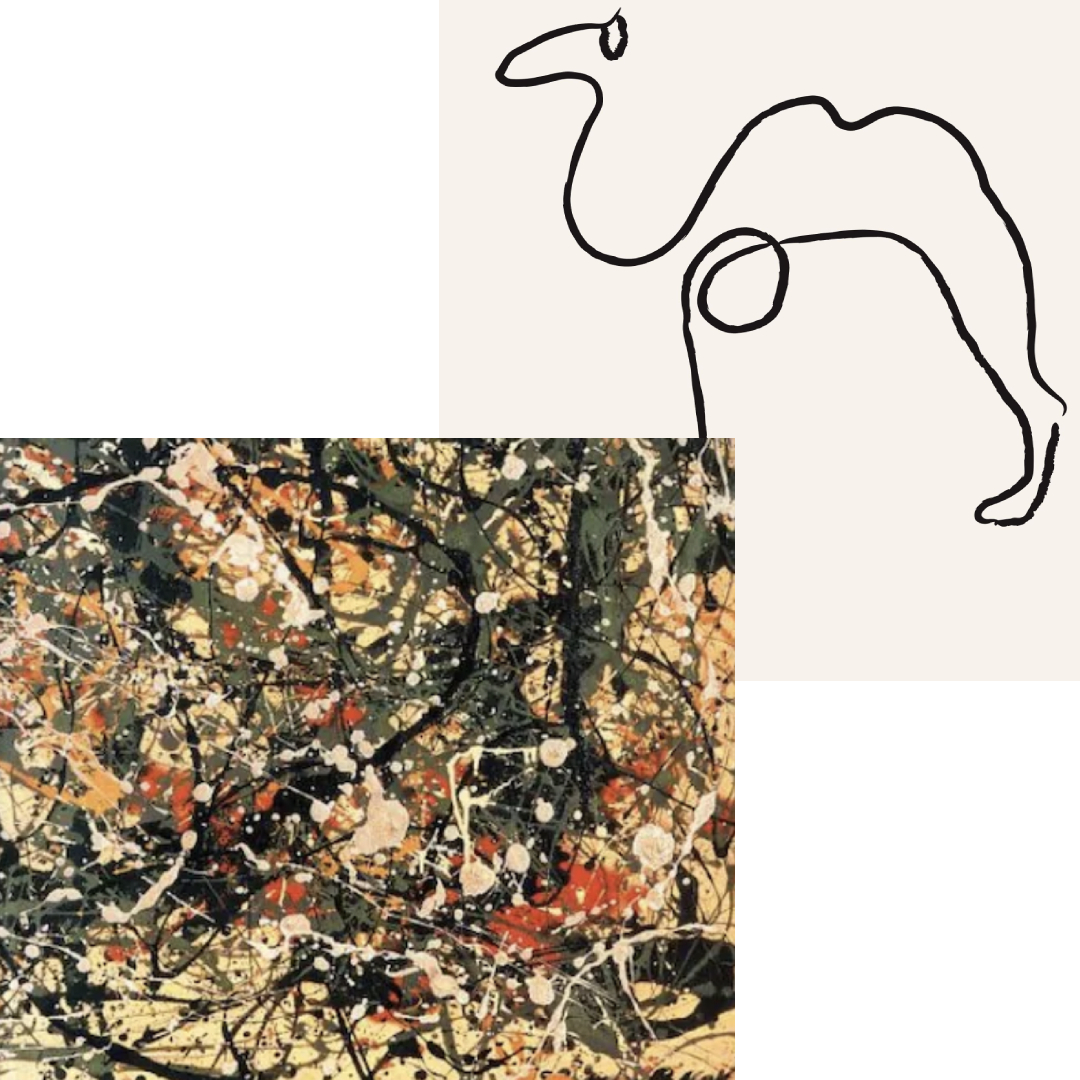
\includegraphics[width=.2\textwidth]{img/logo.jpeg}
}

%\section{Introducere}

%\subsection{Prezentarea generală a disertației}

% FORECAST frame
% ---------------------------------------------------------------------------------

%\begin{frame}[t]{Scopul si tema recurentă în disertație}
%% Main take away that people should remember (MAIN IDEA/forecast)
%% Thesis purpose
%
%Utilizarea metodelor de \alert{inferență bayesiană} pentru a dezvolta și antrena \structure{modele noi} pentru unele dintre cele mai \structure{complexe și profitabile} aplicații din economia managerială:
%
%\visible<1->{
%\begin{enumerate}
%	\item<2-> Măsurarea efectului reclamelor TV asupra vizitelor pe un site web și optimizarea campaniilor de publicitate \footnote{Contribuția principală a disertației e în modelarea bayesiană în marketing}
%	\item<3-> Previziunea cererii pe piața lenjeriei și modei pentru produse noi și serii de timp scurte
%	\item<4-> Modelarea comportamentului consumatorilor în modelul de afaceri contractual ``Try before you buy``
%\end{enumerate}
%}
%
%\visible<5->{
%	abordând \alert{dificultățile econometrice} des întalnite într-un cadru comun al modelării \structure{ierarhice bayesiene}.
%}
%\end{frame}
% ---------------------------------------------------------------------------------

\begin{frame}[t]{}
\centering \shadowbox{(Data-Driven)
	 Decision-Making under Uncertainty, at Scale}
	 
\vspace{5mm}

\begin{columns}
	\begin{column}{0.5\textwidth}
	\begin{block}{Head of Data Science @AdoreMe}
	\begin{itemize}
		\item AI Product Management
		\item Decision Science
		\item Systems' Design
		\item Arhitectura Cloud
	\end{itemize}
	\end{block}
	
	\begin{block}{Aplicatii}
	\begin{itemize}
		\item Sisteme de recomandare
		\item Optimizarea stocurilor
		\item Modele de marketing
		\item Modele de propensitate
	\end{itemize}	
	\end{block}

	\end{column}

	\begin{column}{0.5\textwidth}	
		\begin{figure}[h]
		\scalebox{0.9}{
			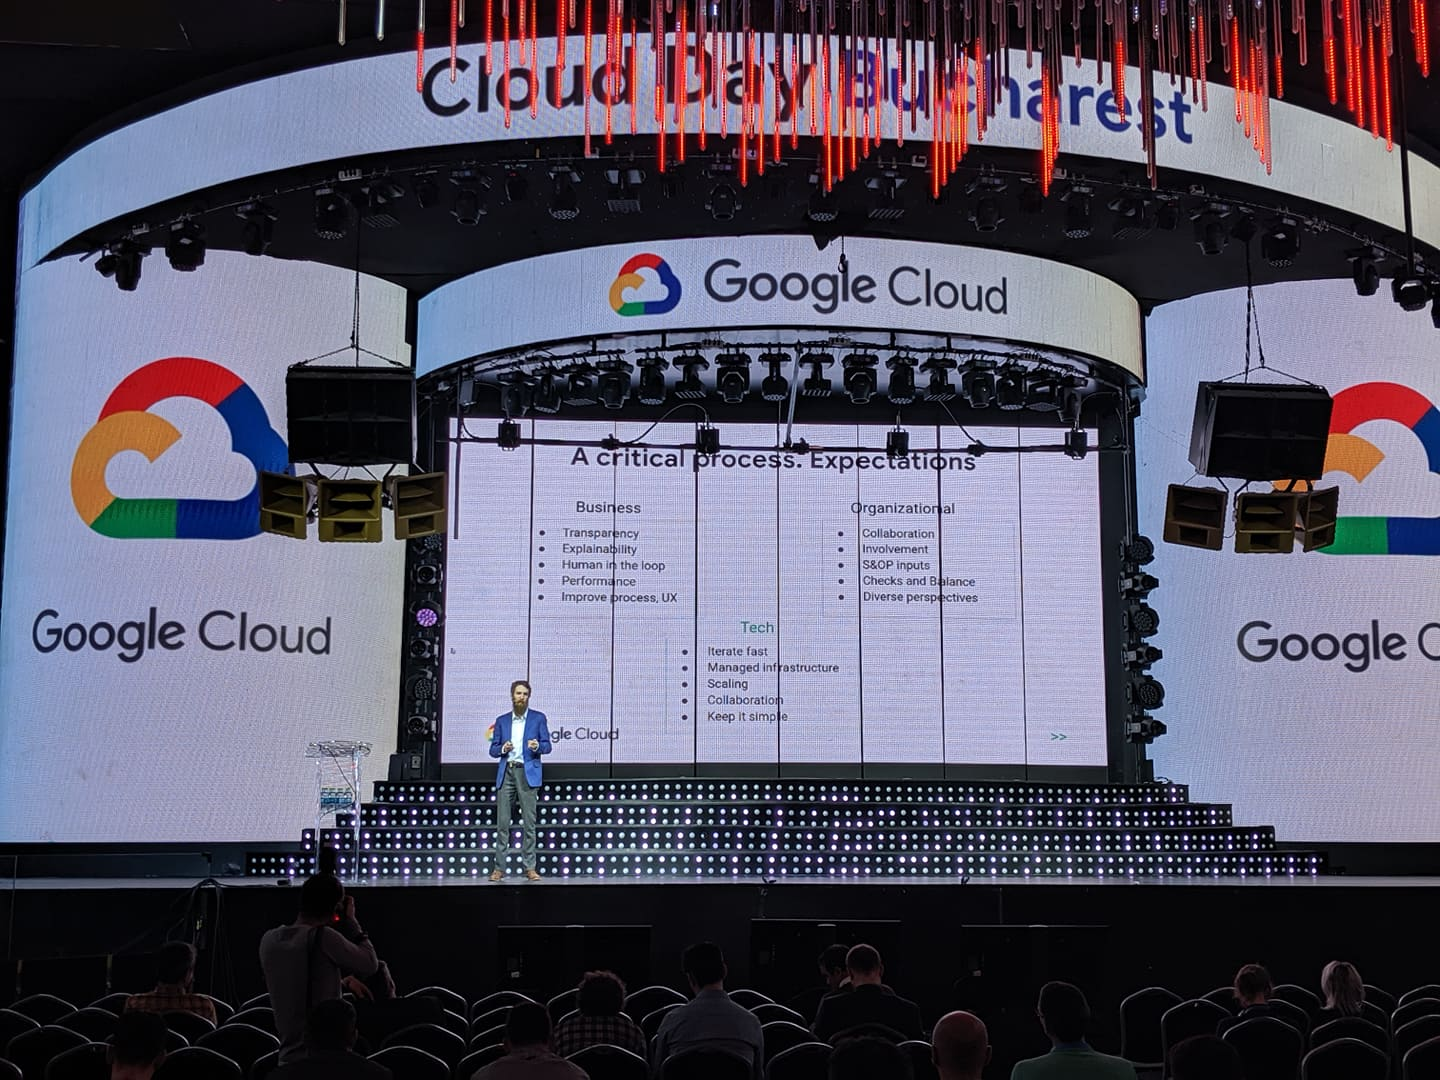
\includegraphics[width=0.9\linewidth]{img/me.jpeg}
		}
		\\ Statistica Bayesiana
		\\ Dinamica sistemelor
		\\ Complexitatea economica
	\end{figure}
	\end{column}
\end{columns}
\end{frame}


\section{Harta Domeniului}

\begin{frame}[t]{Ce as fi vrut de la un curs?}

	\begin{columns}
	\begin{column}{0.5\textwidth}	
		\begin{figure}[h]
		\scalebox{0.9}{
			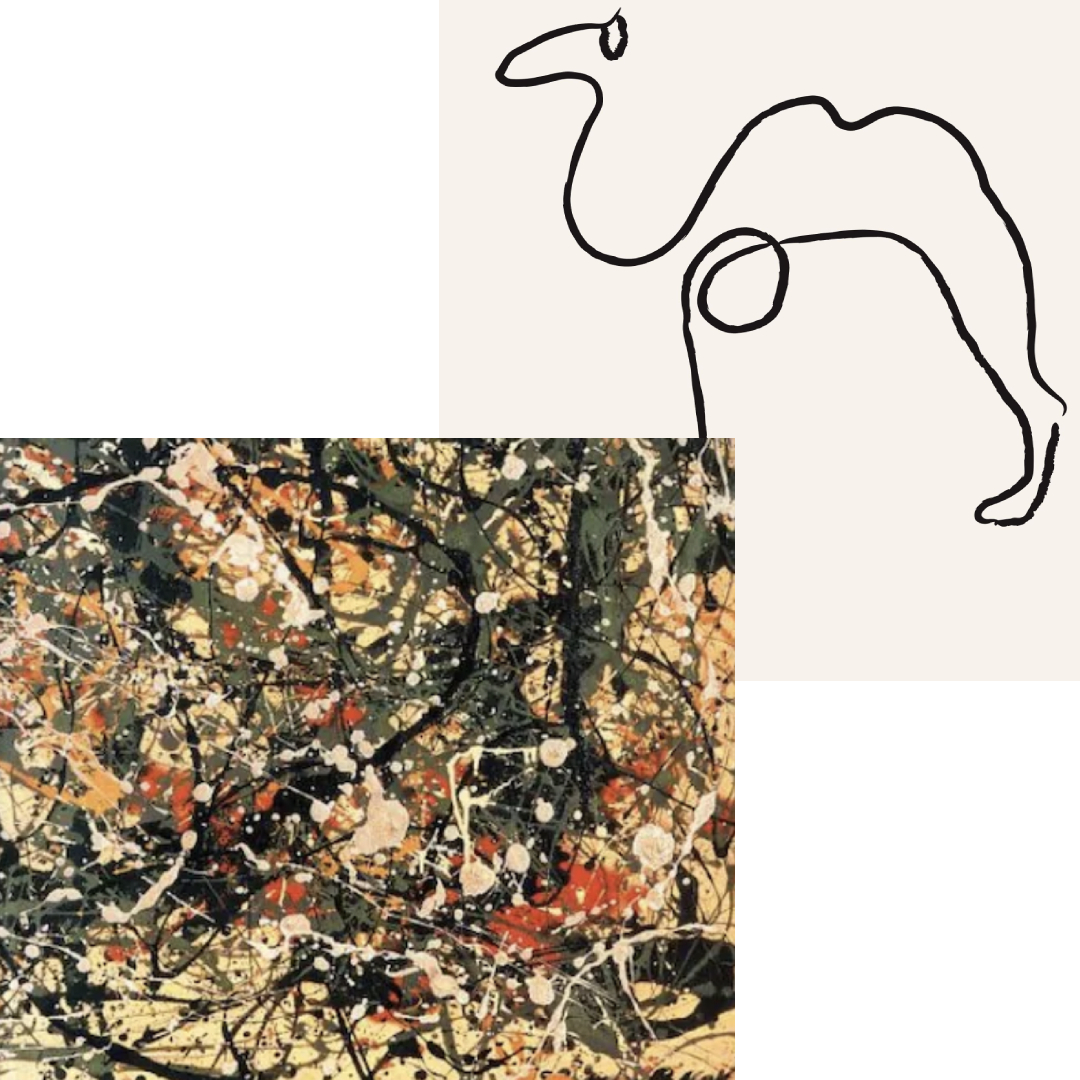
\includegraphics[width=0.9\linewidth]{img/logo.jpeg}
		}
		\\ Realitatea | Date, Regularitati, Zgomot, Esenta
	\end{figure}
	\end{column}
	
	\begin{column}{0.5\textwidth}	
		\begin{itemize}
		\item Motivatie, provocari si aplicatii practice in firme
		\item Intelegere conceptuala si dezvoltarea intuitiei
		\item Simulare, Cod, Vizualizare
		\item Rigoare teoretica
		\item Date apropiate de practica
		\item Implementarea in sisteme reale
	\end{itemize}	
	\end{column}
	\end{columns}
	
\end{frame}
%
%
%\begin{frame}[t]{Importanta Domeniului}
%\end{frame}
%
%
%\begin{frame}[t]{Statistica | Invatare automata | Data Mining}
%	50\% invatare automata | 25\% statistica | 25\% metode exploratorii
%
%\end{frame}

%\begin{frame}[t]{Motivație: dificultăți în microeconometrie}



%\begin{columns}[T]
%	\begin{column}{0.5\textwidth}
%		\structure{Specificul datelor și modelării econometrice} \cite{cameron05}
%		\begin{enumerate}
%			\item<1-> Nivelul scăzut de agregare. Date discrete, neliniare, non netede
%			\item<2-> Mai mult realism și continut informațional. Nivelul individual
%			\item<3-> Eterogenitate și parametri latenți, heteroskedasticitate
%			\item<4-> Dinamica si autocorelarea. Date panel, echilibru stochastic \newline
%		\end{enumerate}
%		\visible<5->{\alert{Probleme comune în cele 3 aplicații!}}		
%	\end{column}
%	
%	
%	\begin{column}{0.5\textwidth}
%		\structure{Caracteristici dorite pentru operaționalizarea modelelor}
%		\begin{enumerate}
%			\item<6-> Învățarea din date și actualizarea modelelor
%			\item<7-> Stabilitatea și robustețea
%			\item<8-> Declararea explicită a ipotezelor stochastice. Combinarea mai multor surse de informații
%			\item<9-> Interpretabilitate, regularizare, selecția variabilelor, pooling
%			\item<10-> Cuantificarea incertitudinii
% 			\item<11-> Metode computaționale eficiente 
%		\end{enumerate}
%
%	\end{column}
%\end{columns}
%%\end{frame}
%
%\begin{frame}[t]{Conexiuni intre domenii. 4 ani in context}
%\end{frame}
%
%
%\begin{frame}[t]{Aplicatii, inovatii}
%\end{frame}
%
%\begin{frame}[t]{Perspective importante}
%\end{frame}
%
%
%
%\begin{frame}[t]{O harta a invatarii automate}
%\end{frame}
%
%
%\begin{frame}[t]{... inteligenta artificiala?}
%\end{frame}
%
%
%\section{Introducere in Invatarea Automata}
%
%\begin{frame}[t]{Procesul de modelare si decizie in firme}
%\end{frame}
%
%
%\begin{frame}[t]{Invatarea automata. Generalizare}
%\end{frame}
%
%\begin{frame}[t]{k-Nearest Neighbors}
%\begin{figure}[ht!]%
%	\subfloat[perceptual importance points]{{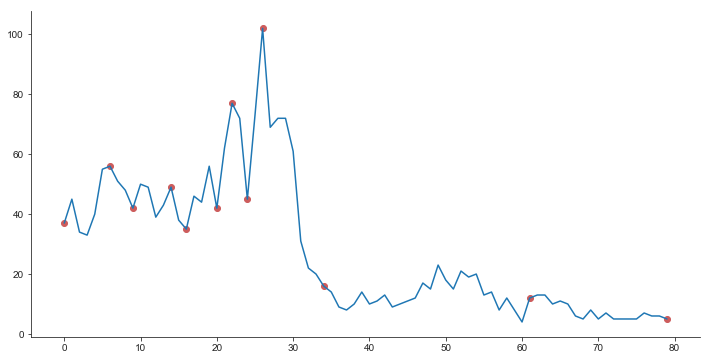
\includegraphics[width=5cm]{img/001.png} }}%
%	\qquad
%	\subfloat[dynamic time wrapping neighbor]{{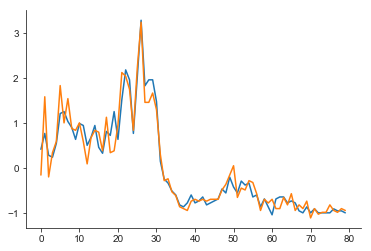
\includegraphics[width=5cm]{img/004.png} }}%
%	\caption{An example of using \textbf{Perceptual Importance Points} applied on a launch pattern of a new products.}
%\end{figure}
%\end{frame}


\end{document}














